\chapter{Space-Efficient, On-the-fly Reachability Analysis} \label{chap:sggen}
\section{Introduction}\label{sec:sgintro}
We have seen that reachability analysis and model checking of TA are
well-established and successful techniques in the analysis of
real-time systems. In Chapter~\ref{chap:tggen}, we have shown how
\bcandle\ models can be translated into TA, and thus have provided a
way by which these verification methods can be applied to \bcandle\
systems. As usual, the state space explosion problem is the major
limiting factor in the use of such techniques, from a technical point
of view. Much current research in TA verification is aimed at
alleviating the worst effects of this problem: in particular,
on-the-fly and symbolic approaches have proven effective in this
respect. In this chapter, we consider how such methods can be adapted for use
in the analysis of \bcandle\ models. 

Traditionally, a system model is presented as a network of small
component TA, and on-the-fly methods, especially, derive their benefit
from the fact that it may be unnecessary to construct their product
automaton completely, before the verification question can be decided.
Unfortunately, in the approach taken in Chapter~\ref{chap:tggen}, it
is necessary to construct a monolithic TA for the system model as a
whole, before verification begins. This is contrary to the spirit of
on-the-fly verification, since, even though the verification problem
may be decided during construction of the simulation graph, the
monolithic TA itself may be very large.  Recall that we need to build
a monolithic TA if we wish to stay within the framework of the
standard timed safety automata (TSA) of Henzinger et
al.~\cite{hnsy:94}, since the product construction for TSA does not
allow a satisfactory modelling of broadcast communication as we have
defined it in Chapter~\ref{chap:bcandle}. It may be possible to define
a translation of \bcandle\ models into networks of TA if we allow the
use of TA extended with data variables and
guards~\cite{alt:98,boz:98,lpy:97}. This would allow us to take
advantage of existing on-the-fly techniques. However, we do not pursue
that line of enquiry in this work, but rather propose a novel solution
to the problem: namely to generate the simulation graph of a system
directly from the extended net created for the construction of its TA,
but \emph{without ever constructing the TA explicitly}. In this way,
we obtain full on-the-fly verification for \bcandle.  Although several
proposals have been published for the verification of real-time
languages by means of translation to
TA~\cite{doy:94,her:98,jm:95,nsy:91}, we believe that this is the
first time that the approach described here has appeared in the
literature.

In addition, we combine on-the-fly verification with a \emph{compact
representation} of the state space. Binary decision diagrams (BDD's)
have been used successfully, mainly in the analysis of hardware
systems where the need for a compact representation of boolean
functions is prevalent~\cite{bry:86}. However, the modelling of
software systems commonly employs a richer set of data types and this
fact motivates the investigation of different encodings of sets of
states than by their characteristic functions. In this chapter, we
consider the use of minimised deterministic finite state automata
(MA's)~\cite{hp:99} for the storage of the set of visited states in
the reachability analysis of \bcandle\ models. This state space
representation promotes sharing of common parts of a set of state
vectors, and seems to be particularly useful in mitigating the effects
of state explosion caused by interleaving in asynchronous models.  So
far as we know, this is the first time that this state compression
technique has been investigated in the analysis of timed systems.

The rest of this chapter is organised as follows: in
\Sec\ref{sec:sgonthefly} the algorithm for on-the fly reachability
analysis is described; minimised automata are introduced in
\Sec\ref{sec:sgma} and their use in the
representation of the set of visited states is described
in~\Sec\ref{sec:sgimpl}; salient features of an experimental platform
are outlined in \Sec\ref{sec:sgplatform} and experimental results are
discussed in~\Sec\ref{sec:sgexperiments}; in~\Sec\ref{sec:sgrelated},
we consider related work; and finally, in~\Sec\ref{sec:sgconc}, we
present our conclusions and suggestions for further work.

\section{On-the-fly reachability analysis}\label{sec:sgonthefly}
\subsection{Basic algorithm}
We consider the problem of determining whether or not it is possible
for a given \bcandle\ system $(\P,\N,\D)$ to reach a state which
satisfies some state formula $\sfmla$. Recall that the
validity of any state formula $\sfmla$ can be determined locally for any 
state $\state$, and that $\state \smodels \sfmla$ denotes the fact
that $\state$ satisfies $\sfmla$. 

In fact, all the machinery needed to solve this problem is already in
place.  The algorithm for constructing a TA from a \bcandle\ system is
given in Figure~\ref{fig:tgmkgraph} and the algorithm for reachability
in the simulation graph of a TA is given in
Figure~\ref{fig:simgraphreach}. Clearly, we can solve our problem by
executing these algorithms consecutively. However, it is straightforward to
combine them into a single algorithm which solves the reachability problem
without explicitly constructing the TA. Such an algorithm is shown in 
Figure~\ref{fig:sgreach}, to which we refer in the following explanatory
comments.

We assume that $(\PP,\NN,\D)$ is a safely clocked \bcandle\ system
and that $\cmax(\PP,\NN,\D)$ gives the value of the largest constant
appearing in a computation $[\op:t_1,t_2]$ in $\PP$, or a message
transmission latency bound $\dub(\mm)$, $\duB(\mm)$ in $\NN$. The net
$\RR = (\W,\T,\WI)$, given by $\mknet{\PP}$, is constructed as
described in~\Sec\ref{sec:consnet}. We wish to check whether a state
satisfying the state formula $\sfmla$ is reachable from the initial
state comprising the location $\tgiloc = (\WI,\NN,\D)$ and the clock zone
$\suc{\tau}{\tgiloc}(\cczero)$.  The rest of the algorithm shows a
standard depth-first or breadth-first search of the reachable state
space. The only section warranting further comment concerns the
calculation of successor states at lines (14--15).  Notice here that a
location $\tgloc$ is of the form $(\W,\NN,\D)$ and that the relation $\tgloc
\goesr{\tgguard,\any,\resets} \tgloc'$ yields successor locations
$\tgloc' = (\W',\NN',\D')$ according to the rules \textbf{R.1} and
\textbf{R.2}~(Definition~\ref{def:tgnetrules}). Each such
successor determines an edge $\tgedge =
(\tgloc,\tgguard'',\any,\resets,\tgloc')$ which can be used in the
calculation of the clock zone successors of $\vexcond$ in the
usual way: $\vexcond' =
\close{c}{\suc{\tau}{\tgloc'}(\suc{\tgedge}{}(\vexcond))}$. This allows
the algorithm to follow the usual pattern for simulation graph
reachability (Figure~\ref{fig:simgraphreach}).
 
\begin{figure}
\begin{center}
\small
\NumberProgramstrue
\begin{programbox}
\INPUT
  \text{initial system } (\PP,\NN,\D), c = \cmax(\PP,\NN,\D)
  \text{net } \RR = (\W,\T,\WI) = \mknet{\PP}
  \text{state formula } \sfmla
\ENDINPUT
\BEGIN 
  \tgiloc := (\WI,\NN,\D)
  |VISITED| := \{(\tgiloc, \suc{\tau}{\tgiloc}(\cczero))\}
  |WAITING| := \{(\tgiloc, \suc{\tau}{\tgiloc}(\cczero))\}
  \WHILE |WAITING| \neq \emptyset \DO
    \text{remove some } (\tgloc,\vexcond) \text{ from }  |WAITING|
    \IF (\tgloc,\vexcond) \smodels \sfmla
    \THEN \RETURN \text{ `yes' }
    \ELSE
      |succ| := \{(\tgloc',\vexcond') \vbar \tgloc \goesr{\vexcond'',\any,\resets} \tgloc' \land \tgedge = (\tgloc, \vexcond'', \any, \resets, \tgloc') \land
  \t2 \vexcond' = \close{c}{\suc{\tau}{\tgloc'}(\suc{\tgedge}{}(\vexcond))} \neq \emptyset\}
      \FOREACH (\tgloc_s,\vexcond_s) \in |succ| \DO
        \IF (\tgloc_s,\vexcond_s) \notin |VISITED|  
          \text{add } (\tgloc_s,\vexcond_s)\ \text{ to } |VISITED|
          \text{add } (\tgloc_s,\vexcond_s)\ \text{ to } |WAITING|
        \FI  
      \OD
    \FI
  \OD
  \RETURN \text{ `no' }
\END
\end{programbox}
\end{center}
\caption{Algorithm for on-the-fly reachability for \bcandle \label{fig:sgreach}}
\end{figure}

\subsection{Clock activity reduction}\label{ss:sgact}
The memory requirements of the basic on-the-fly reachability algorithm
can be reduced considerably by reducing the number of clock variables
which are used in the model to be analysed.  Daws and
Yovine~\cite{dy:96} have proposed an important technique, known as
\emph{clock activity} reduction, which ensures that only the \emph{active}
clocks are recorded in each symbolic state in the simulation graph. A
clock is considered to be active if its value will be \emph{tested}
before it is next \emph{reset}. It is clear that there is no need to
record the values of the other clocks, since they can have no effect
upon the behaviour of the system until their current values have been
destroyed by a clock reset. The remainder of this section shows how 
clock activity reduction can be employed in the on-the-fly reachability
algorithm for \bcandle.

\subsubsection{Active clocks} 
Let $\AA$ be a TA with set $\tglocs$ of locations, set $\clocks$ of
clocks and set $\tgedges$ of edges.  Define an \emph{edge path} of
length $n$, over $\tgedges$, to be a sequence $\epath$ of edges,
$\tgedge_0,\tgedge_1,\ldots,\tgedge_{n-1}$, where $n \in \nat$,
$\tgedge_i \in \tgedges$, and, for $0 < i < n$, $\esource(\tgedge_{i}) 
= \etarget(\tgedge_{i-1})$.  Let
$\Epath$ denote the set of edge paths over $\tgedges$, and
$\length{\epath}$ denote the length of edge path $\epath \in \Epath$.

We say that a clock $\clock \in \clocks$ is \emph{tested} in
location $\tgloc \in \tglocs$, if $\clock$ occurs in the invariant
$\tginv(\tgloc)$ or in the guard of some outgoing edge of $\tgloc$.
We denote by $\tclk(\tgloc)$ the set of clocks tested in $\tgloc$.  A
clock $\clock$ is said to be \emph{active} in location
$\tgloc$ iff it is either tested in $\tgloc$ or is tested
in some location $\tgloc' \in \tglocs$ which is connected to $\tgloc$ by
an edge path along which $\clock$ is never reset. 
\begin{definition}[Active clocks]\label{def:sgactiveclocks}
Let $\AA = (\tglocs,\tgiloc,\Actions,\tgclks,\tgedges,\tginv)$ be a TA.
Let $\tclk : \tglocs \fun 2^\tgclks$ define, for each location $\tgloc
\in \tglocs$, the set of clocks occurring either in the invariant 
$\tginv(\tgloc)$, or in the clock constraint of some outgoing edge of $\tgloc$.
Then, for any location $\tgloc \in \tglocs$,
the set of \emph{active clocks} of $\tgloc$ is denoted $\act(\tgloc)$, and
is defined by 
\[ \act(\tgloc) \defs \tclk(\tgloc) \cup \nreset(\tgloc) \] 
where a clock $\clock$ is in 
$\nreset(\tgloc)$ iff $\clock$ is not tested in $\tgloc$ but
is tested in some location connected to $\tgloc$ by an edge path 
along which $\clock$ is never reset, i.e. \\
\hspace*{2cm}
$\nreset(\tgloc) \defs \{\clock \in \tgclks | \clock \notin \tclk(\tgloc) 
  \land$ \\
\hspace*{4cm} 
$(\exists \epath \in \Epath, \tgloc' \in \tglocs \such  
\tgloc = \esource(\tgedge_0) \land  
\tgloc' = \etarget(\tgedge_{\length{\epath}-1}) \land$ \\ 
\hspace*{4cm}
$\clock \in \tclk(\tgloc') \land 
\clock \notin \bigcup_{0 \leq i < \length{\epath}} \ereset(\tgedge_i))\}$
\qed
\end{definition}

\subsubsection{Activity graph}
An activity function $\act : \tglocs \fun 2^\tgclks$ can be used in a
\emph{dimension-restricting} projection of the convex
$\clocks$-polyhedron $\vexcond$, occurring in a symbolic state
$(\tgloc,\vexcond)$, in order to produce a new symbolic state
$(\tgloc,\vexcond')$, where $\vexcond'$ is a polyhedron on
$\act(\tgloc) \subseteq \clocks$ instead of on $\clocks$. If
$\act(\tgloc) \subset \clocks$, then the DBM representation of
$\vexcond'$ can be smaller than the representation of $\vexcond$.  In
practice, for a TA constructed from a \bcandle\ description, as
described earlier, the savings are usually very significant and allow
the analysis of many models which would be intractable without
this reduction.
\begin{definition}[Dimension restricting projection~\cite{tri:98}] 
\mbox{\strut} \\ 
Given a $\clocks$-polyhedron $\vexcond$ and a subset of clocks
$\someclks \subseteq \clocks$, the \emph{dimension-restricting}
projection of $\vexcond$ to $\someclks$, denoted
$\clkrestrict{\vexcond}{\someclks}$, is the $\someclks$-polyhedron
$\vexcond'$ such that \\
\hspace*{2cm} $\clkvl' \in \vexcond' \text{ iff } 
   \exists \clkvl \in \vexcond \such \forall \clock \in \someclks
   \such \clkvl(\clock) = \clkvl'(\clock)$
\qed
\end{definition}
\begin{definition}[Activity Graph~\cite{tri:98}]\label{def:sgactivitygraph} 
Let $\AA = (\tglocs,\tgiloc,\Actions,\tgclks,\tgedges,\tginv)$ be a TA
with $c \geq \cmax(\AA)$. Let $\act : \tglocs
\fun 2^\tgclks$ be an activity function for $\AA$. 
The \emph{activity graph} of $\AA$ with respect to $c$, starting at
the symbolic state $\z_0$, is denoted $\AG(\AA,c,\z_0)$, and is
obtained from the simulation graph $\SG(\AA,c,\z_0)$ by the following
modification:
\begin{itemize}
\item For each node $(\tgloc,\vexcond)$ of $\SG(\AA,c,\z_0)$, the node
  $(\tgloc, \clkrestrict{\vexcond}{\act(\tgloc)})$ is a node of 
  $\AG(\AA,c,\z_0)$
\item For each edge $(\tgloc,\vexcond) \goes{a} (\tgloc',\vexcond')$
  of $\SG(\AA,c,\z_0)$, $(\tgloc,\clkrestrict{\vexcond}{\act(\tgloc)})
  \goes{a} (\tgloc',\clkrestrict{\vexcond'}{\act(\tgloc')})$ is an edge
  of $\AG(\AA,c,\z_0)$.
\qed
\end{itemize}
\end{definition}

\begin{notation}
The activity graph of $\AA$ with respect to $c$, starting at the initial 
state $(\tgiloc,\cczero)$, is denoted simply by $\AG(\AA,c)$, and
$\AG(\AA)$ denotes $\AG(\AA,\cmax(\AA))$.
\end{notation}

Tripakis~\cite{tri:98} shows that the activity graph preserves the
same properties as the simulation graph. In particular, the
correctness theorem~(Proposition~\ref{prop:simgraph}) is preserved,
and so we can safely use the activity graph to decide reachability
properties. In fact, it is trivial to modify the algorithm of
Figure~\ref{fig:sgreach} to achieve this. We simply replace the
calculation of successors (lines 14--15) so that each clock zone is
restricted to the active clocks, as follows
\begin{zed}
      succ := \{(\tgloc',\clkrestrict{\vexcond'}{\act(\tgloc')}) | \tgloc \goesr{\vexcond'',\any,\resets} \tgloc' \land \tgedge = (\tgloc, \vexcond'', \any, \resets, \tgloc') \land \\
  \t2 \vexcond' = \close{c}{\suc{\tau}{\tgloc'}(\suc{\tgedge}{}(\vexcond))} \neq \emptyset\}
\end{zed}

\subsubsection{Calculating active clocks in \bcandle}
In~\cite{dy:96}, an algorithm is given to compute the activity function
$\act$ from the syntactic structure of a single TA modelling the entire 
system. It is shown in~\cite{dt:98} how to compute and apply $\act$ on-the-fly,
during construction of the simulation graph of the parallel composition
of a set of TA. In order for activity reduction to be useful in the
reachability analysis of \bcandle, it is necessary to achieve a similar
on-the-fly computation of $\act$. We see from the modification above,
to the on-the-fly algorithm for \bcandle, that the only point at which
$\act$ is required is during the calculation of successors, when,
given an edge $\tgedge = (\tgloc,\_,\_,\_,\tgloc')$,
we need to be able to compute $\act(\tgloc')$. Before considering the 
calculation of active clocks, we first identify the clocks which are tested
in a given location.

A location $\tgloc$, in the TA of a \bcandle\ system, is a tuple
$(\W,\NN,\D)$. The set of \emph{tested} clocks of
such a location is defined below.
\begin{definition}[Tested Clocks]\label{def:sgtclk}
Let $\csys \in \CSys{}$ be a clocked \bcandle\ system and $\GrImpl(\csys)
= (\tglocs,\tgiloc,\Actions,\clocks,\tgedges,\tginv)$
the TA constructed by Definition~\ref{def:tgconstructautomaton}. 
Let $(\W,\NN,\D) \in \tglocs$. The \emph{tested} clocks of
$(\W,\NN, \D)$ are denoted $\tclk(\W,\NN,\D)$, where
\begin{eqnarray*}
\tclk(\W,\NN,\D) & \defs & \tclk(\W,\D) \cup \tclk(\NN) \\
\tclk(\W,\D) & \defs & \bigcup_{\ww \in \W} \tclk(\tattrib\tr_\ww, \D) \\
\tclk(\kk!\ii.\xx,\D) & \defs & \{\uclock\} \\
\tclk(\kk?\ii.\xx,\D) & \defs & \emptyset \\
\tclk([\op:\ti_1,\ti_2]^\clock,\D) & \defs & \ite{\ti_1 \in \nat \lor \ti_2 \in \nat}{\{\clock\}}{\emptyset} \\
\tclk(\gu{\g},\D) & \defs & \ite{\D \models \g}{\{\uclock\}}{\emptyset} \\
\tclk(\NN) & \defs & \bigcup_{\kk \in \K} \tclk(\NN_\kk) \\
\tclk(\free,\emq)^\clock & \defs & \emptyset \\
\tclk(\free,\mm\cq\mq)^\clock & \defs & \{\uclock\} \\
\tclk(\preact{\ti_1,\ti_2}{\mm},\mq)^\clock & \defs & \ite{\ti_1 \in \nat \lor \ti_2 \in \nat}{\{\clock\}}{\emptyset} \\
\tclk(\offers{\mm},\mq)^\clock & \defs & \{\uclock\} \\
\tclk(\postact{\ti_1,\ti_2}{\mm},\mq)^\clock & \defs & \ite{\ti_1 \in \nat \lor \ti_2 \in \nat}{\{\clock\}}{\emptyset}
\end{eqnarray*}   
\qed
\end{definition}
It is easy to see that a clock $\clock$ appears in the invariant, or
the guard of an outgoing edge, of a location $(\W,\NN,\D)$ iff $\clock \in
\tclk(\W,\NN,\D)$.  This follows directly from the definitions of
$\tclk$, rules \textbf{R.1} and \textbf{R.2}~(Definition~\ref{def:tgnetrules})
and the invariant function~(Definition~\ref{def:tgconstructautomaton}).

Now we observe that, in fact, for any location $\tgloc = (\W,\NN,\D)$,
the set of clocks \emph{active} in $\tgloc$ is identical to the set of clocks
\emph{tested} in $\tgloc$.
 
\begin{proposition} \mbox{\strut} \\
Let $\csys \in \CSys{}$ be a clocked \bcandle\ system and $\GrImpl(\csys) =
(\tglocs, \tgiloc, \Actions, \tgclks, \tgedges, \tginv)$ its TA. Then, for any
$\tgloc \in \tglocs$, it is the case that $\act(\tgloc) = \tclk(\tgloc)$.
\end{proposition}
\begin{proof}
By definition, $\act(\tgloc) = \tclk(\tgloc) \cup \nreset(\tgloc)$.  We show
that $\nreset(\tgloc) = \emptyset$, for any $\tgloc \in \tglocs$.  
The following lemma is required: 
\begin{lemma}
For any clock $\clock \in \clocks$ and any edge $\tgedge \in \tgedges$, if
$\clock \notin \tclk(\esource(\tgedge))$ and 
$\clock \in \tclk(\etarget(\tgedge))$, then $\clock \in \ereset(\tgedge)$
\end{lemma}
\begin{proof}
Let $\esource(\tgedge) = (\W_1,\NN,\D)$ and $\etarget(\tgedge) =
(\W_2,\NN',\D')$. Observe that $\tgedge$ must be derived using one of the rules
\textbf{R.1} or \textbf{R.2}. We consider a clock $\clock \in
\clocks$ such that $\clock \notin \tclk(\W_1,\NN,\D)$ and either $\clock \in
\tclk(\W_2,\D')$ or $\clock \in \tclk(\NN')$. We show that 
$\clock \in \ereset(\tgedge)$. There are two cases to consider.
\begin{trivlist}
\item[\it (Case $\clock \in \tclk(\W_2,\D')$)]  
By definition, $\tclk(\W_2,\D') = \bigcup_{\ww_2 \in
\W_2} \tclk(\tattrib\tr_{\ww_2},\D')$.  By \textbf{R.1}, we have that for all 
$\ww_2 \in \W_2$, either there is some $\ww_1 \in \W_1$ and transition
$\tr_{\ww_1} = (\ww_1,\WV,\tattrib,\WT)$ such that $\ww_2 \in \WT$, or
$\ww_2 \in \W_1 \setminus \WT$.  If $\ww_2 \in \WT$ then, since
$\tclk(\WT ,\D') \subseteq \clk(\WT) \subseteq \ereset(\tgedge)$, we
have $\clock \in \ereset(\tgedge)$.
On the other hand, if $\ww_2 \in \W_1 \setminus \WT$, then $\clock
\syneq \uclock$; this must be so since, by assumption, $\clock \notin
\tclk(\W_1,\D)$, and, therefore, must be tested in $\D'$ by reason of the fact
that $\tattrib\tr_{\ww_2} = \gu{\g}$ for some data guard $\g$ such that
$\D \not\models \g$ and $\D' \models \g$. Since the urgent clock 
is reset on every edge, again, we have $\clock \in \ereset(\tgedge)$.
\item[\it (Case $\clock \in \tclk(\NN')$)] If $\clock \in \tclk(\NN')$ then 
either $\clock \syneq \clock_\kk$, for some
channel identifier $\kk$, such that $\NN_\kk = (\_,\clock_\kk)$, or 
$\clock \syneq \uclock$. 
If $\clock_\kk \notin \tclk(\NN)$ and $\clock_\kk \in \tclk(\NN')$
then $\tgedge$ must be derived by \textbf{R.2} using either \textbf{E\_N.1} or
\textbf{E\_N.3}. In both cases, $\clock \syneq \clock_\kk \in 
\ereset(\tgedge)$. On the other hand, if $\clock \syneq \uclock$, then 
$\clock \in \ereset(\tgedge)$. In either case, the result follows.
\end{trivlist}
\end{proof}
Now, observe that $\nreset(\tgloc) = \bigcup_{n \geq 0} \nreset_n(\tgloc)$,
where $\nreset_0(\tgloc) \defs \emptyset$, and, for $n > 0$,
\begin{zed}
\nreset_n(\tgloc) \defs \{\clock \in \tgclks | \clock \notin \tclk(\tgloc) \land \\
\t2 (\exists \epath \in \Epath, \tgloc' \in \tglocs \such  
\length{\epath} = n \land \tgloc = \esource(\tgedge_0) \land  \tgloc' = \etarget(\tgedge_{n-1}) \land \\ \t3 \clock \in \tclk(\tgloc') \land 
\clock \notin \bigcup_{0 \leq i < n} \ereset(\tgedge_i))\}
\end{zed}
The proof of the proposition then follows by induction on the 
length of an $\Epath$.
\end{proof}

This result has significant implications for the efficiency of the
analyses which can be performed on \bcandle\ systems, which surpasses
that which can be achieved for general TA models where this property
may not be exhibited. Most significantly, the result justifies the use
of $\tclk$ as the activity function in the construction of the
activity graph. Clearly, $\tclk$ can be calculated locally for any
given location and, therefore, can be implemented efficiently and
applied on-the-fly to achieve clock activity reduction during
construction of the graph. The experimental data presented in
\Sec\ref{sec:sgexperiments} and \Sec\ref{ss:prexampleanal} provides evidence 
for the utility of this technique in practice.
 
\section{A Minimised Automaton Representation of Reachable States\label{sec:sgma}}
Even with the clock activity reduction described in the previous
section, the size of the state space, which arises in the analysis of
a system model, can grow too big to be stored in computer
memory. There are many proposals in the literature for reducing the
memory required to store a set of states --
see~\Sec\ref{sec:sgrelated}. In this section, we consider an approach
in which a state vector is regarded as being encoded as a string over
some alphabet, and the set of visited states is represented by a
minimised deterministic finite automaton (MA) which recognises the
language comprising the set of state vector strings.  This technique
has been implemented in the model checker SPIN~\cite{hp:99}, where it
has been shown to achieve even better compression for many systems
than that obtained by the use of BDD's~\cite{vis:96}. Similar results
have been reported in experiments using \emph{sharing
trees}~\cite{ggz:95,zam:97} (also known as
\emph{GE-SETS}~\cite{gre:96}); the implementation of the sharing tree data
structure is very similar to the MA implementation described here.  By
comparison with other techniques which also ensure complete state space
coverage, the space reductions achieved by the use of MA's are among
the best reported in the literature. It is of considerable interest to
see if this performance is observed also in the storage of the state
spaces which arise in the analysis of timed systems. Our work is the
first to report such experiments.

In the remainder of this section, we introduce the basic ideas and definitions
for the use of MA's in state space storage. Later, we discuss
their application in the implementation of a state store for \bcandle.

\subsection{Minimised Deterministic Finite State Automata}\label{ss:sgma}
\begin{definition}
A $k$-layer \emph{deterministic finite state automaton} (DFA) is a
tuple $\MA = (\MAstates,\MAalphabet,\MAtr)$ where 
\begin{itemize}
\item 
$\MAstates = \bigcup\{\MAstates_i | 0 \leq i \leq k\}$ is the set of
states. $\MAstates_i$, $\emptyset \subset \MAstates_i \subset
\MAstates$, is the set of states at the $i$th layer and $\MAstates_i
\cap \MAstates_j = \emptyset$ for $i \neq j$.  $\MAstates_0$ is a
singleton containing the initial state and $\MAstates_k =
\{\MAT,\MAF\}$, where $\MAT$ is the accepting final state and $\MAF$
is the rejecting final state. The set $\MAstates
\setminus \MAstates_k$ is denoted $\MAstates^-$. 
\item
$\MAalphabet$ is the alphabet.
\item
$\MAtr : \MAstates^- \cross \MAalphabet \fun \MAstates$ is a total
function such that for all states $\MAstate \in \MAstates^-$ and
symbols $\MAsymb \in \MAalphabet$, if $\MAstate \in \MAstates_i$ then
$\MAtr(\MAstate,\MAsymb) \in \MAstates_{i+1}$.
\qed
\end{itemize}
\end{definition}
A \emph{string} $\MAstring$ of \emph{length} $n$ is a sequence of
symbols $\MAstring = \MAsymb_0,\MAsymb_1,\ldots,\MAsymb_{n-1}$, where
$\MAsymb_i \in \MAalphabet$ for $0 \leq i < n$. $\MAalphabet^n$
denotes the set of strings of length $n$ over the alphabet 
$\MAalphabet$. A string $\MAstring =
\MAsymb_0,\MAsymb_1,\ldots,\MAsymb_{n-1}$ \emph{generates a state
sequence} $\MAstate_0,\MAstate_1,\ldots,\MAstate_n$ from state
$\MAstate = \MAstate_0$, where $\MAstate_{j+1} =
\MAtr(\MAstate_j,\MAsymb_j)$ for $0 \leq j < n$.  For a state
$\MAstate \in \MAstates_i$, we denote the \emph{language of} $\MAstate$ by
$\Lang_\MA(\MAstate)$. $\Lang_\MA(\MAstate)$ is the set of strings
which generate a state sequence from $\MAstate$ ending with the terminal 
state $\MAT$. 
Formally, for $\MAstate \in \MAstates_i$,
\begin{zed}
\Lang_\MA(\MAstate) \defs \{\MAstring
\in \MAalphabet^{k-i} | \MAstring \text{ generates the state sequence }
\MAstate_0,\MAstate_1,\ldots,\MAstate_{k-i} \\
\t2 \text{ from } \MAstate, \text{ and } \MAstate_{k-i} = \MAT\}
\end{zed}
We define $\Lang(\MA) = \Lang_\MA(\MAstate_0)$ where $\MAstate_0 \in
\MAstates_0$.  A DFA is \emph{minimised} provided $\Lang(\MAstate_i) =
\Lang(\MAstate_j)$ iff $\MAstate_i = \MAstate_j$.

\begin{exampleb}
The MA of Figure~\ref{fig:ma} is $\MA =
(\{\MAstates_i\}_{i=0}^4,\MAalphabet,\MAtr)$, where $\MAstates_0 =
\{0\}, \MAstates_1 = \{1,2,3\}, \MAstates_2 = \{4,5\}$, $\MAstates_3 =
\{6,7\}$ and $\MAstates_4 = \{\MAT,\MAF\}$ is the set of states;
$\MAalphabet = \{a,b,c\}$ is the alphabet; and $\MAtr$ is the set of edges
as shown in the figure. $\MA$ represents the set $S \subseteq
\MAalphabet^4$ of strings where
\begin{eqnarray*}
S & = & \{aaaa,aaba,aaca,abaa,abba,abca,acaa,acba,acca, \\
&&        baab,baba,baca,bbab,bbba,bbca,bcaa,bcba,bcca, \\
&&        caab,caba,caca,cbaa,cbba,cbca,ccab,ccba,ccca\}
\end{eqnarray*}
\qed  
\end{exampleb}
\begin{figure}
\begin{center}
\includegraphics[width=.8\linewidth]{SGGEN/ma.eps}
\end{center}
\caption{A minimised automaton\label{fig:ma}}
\end{figure}

It can be seen that a MA achieves a compact representation of a set of
strings by a combination of \emph{prefix merging} and \emph{suffix
merging}.  The requirement that a MA is deterministic ensures that all
shared prefixes are recorded only once. Similarly, the requirement of
minimisation ensures that many shared suffixes are also recorded only
once. Furthermore, for any MA, the amount of sharing in prefixes and
suffixes is optimal, in the sense that any other MA recording the same
information is guaranteed to be isomorphic. In fact, a MA gives a canonical
representation of a language -- there is only one MA (up to
isomorphism) representing a given language, and different languages
are represented by different MA's~\cite{hu:79}. An effective use of
MA's for state space representation will require that state vectors
are organised so as to promote as much prefix and suffix merging as
possible.  It is worth noting that the compactness of sharing trees
(GE-SETS) relies on the same idea. The relationship between MA's and
sharing trees is discussed in~\cite{zam:97}.
 
\subsubsection{MA Operations}
There are three basic operations on MA's which are required to implement 
a state store for reachability analysis: 
\begin{description}
\item[initialise] -- create a MA $\MA$ having an
empty language, i.e., ensure $\MA$ satisfies $\Lang(\MA) = \emptyset$; 
\item[insert] -- given a MA $\MA$ and a string $\MAstring$, create a
MA $\MA'$ such that $\Lang(\MA') = \Lang(\MA) \cup \{\MAstring\}$;
\item[member] -- given a MA $\MA$ and a string $\MAstring$, return
  $\True$ if $\MAstring \in \Lang(\MA)$, otherwise return $\False$.  
\end{description}
Holzmann and Puri~\cite{hp:99} give efficient algorithms for each of
these operations.  To be precise, for a $k$-layer MA $\MA$ over an
alphabet $\MAalphabet$, their {\bf insert} algorithm is
$\bigO(k\modulus{\MAalphabet})$, {\bf member} is $\bigO(k)$ and {\bf
initialise} is $\bigO(1)$.  We refer the reader to the cited work for
a detailed description of the algorithms.
  

\section{Implementing a MA state store for \bcandle\label{sec:sgimpl}}
In order to use a MA for the state store in a reachability analysis of
a \bcandle\ system, it is necessary to partition the state vector and
allocate partitions to layers in the MA. How this is done can have a
significant effect upon the efficiency of the state store. In this
section, we discuss the structure of a \bcandle\ state vector and
consider some principles which may be applied in determining an
effective partitioning.

\subsection{The state vector}
A \bcandle\ state vector has the general form shown in
Figure~\ref{fig:sgsvec}, where it can be seen that a state vector
represents a location $\tgloc = (\W,\NN,\D)$ and a clock zone
$\vexcond$. The representation is discussed in more detail below.
\begin{figure*}
\begin{center}
\begin{tabular}{|l|l|l|}
\hline
& Marking ($\W$) & $\{\ww_1,\ww_2,\ldots,\ww_m\}$ \\ 
\cline{2-3}
LOCATION ($\tgloc$) & Network ($\NN$) & $\{(\ss_1,\mq_1),(\ss_2,\mq_2),\ldots,(\ss_n,\mq_n)\}$\\ 
\cline{2-3} 
& Data ($\D$) & $\{\vv_1,\vv_2,\ldots,\vv_d\}$  \\ 
\hline
ZONE ($\vexcond$) & \multicolumn{2}{c|}{$\{\bb_1,\bb_2,\ldots,\bb_z\}$} \\ 
\hline  
\end{tabular}
\end{center}
\caption{Structure of a \bcandle\ state vector \label{fig:sgsvec}}
\end{figure*}
\begin{description}
\item[Marking] The marking $\W = \{\ww_1,\ww_2,\ldots,\ww_m\}$ is the set of
marked places of the system net~(\Sec\ref{ss:tgnets}) which represents the
state of the system processes. 
\item[Network] For each channel in the system network, its
dynamically changing components are recorded in the state vector, i.e., 
the status $\ss$ and the queue $\mq$ of messages pending transmission. 
The status
consists of one of the four values $\FREE, \PRE, \ACCEPT$, or $\POST$,
and, optionally, an associated message, comprising a message
identifier and a data value. The message queue can be modelled in a variety
of ways. In the following, we will assume a fixed length sequence of messages.
\item[Data] Let $\Var = \{\xx_1,\xx_2,\ldots,\xx_d\}$ be the set of data
variables, where each variable $x_i$ ranges over a domain of values,
$\V_{\xx_i}$. The
data environment $\D$ is represented by recording its valuation
function $\val = \{\xx_1 \mapsto \vv_1, \xx_2 \mapsto \vv_2,\ldots,\xx_d \mapsto \vv_d\}$. This is done simply by fixing the 
order of the variables and storing the corresponding values 
$\{\vv_1,\vv_2,\ldots,\vv_d\}$. 
\item[Zone] 
The clock zone $\vexcond$ is represented as a
DBM~(\Sec\ref{ss:mscdbm}), i.e. a set of bounds $\{\bb_1,\ldots,\bb_z\}$. 
Here, the main issue is how to take advantage
of clock activity reduction in order to reduce the storage
requirements.  For example, consider a TA $\AA$ with clock set
$\clocks = \{\clock_1,\clock_2, \ldots, \clock_7\}$, whose set of
reachable states contains no state in which more than 3 clocks are
active simultaneously, and many states which have fewer than 3
active clocks.
\begin{figure}
\begin{center}
\begin{tabular}{cc}
\multicolumn{2}{c}{
\begin{tabular}{|>{$}c<{$}|>{$}c<{$}>{$}c<{$}>{$}c<{$}>{$}c<{$}|}
\hline
\M  & 0        & 1         & 2         & 3         \\
\hline
0   & 4        & (-3,\leq) & (-5,\leq) & (-2,\leq) \\
1   & (7,\leq) & \clock_2  & (2,\leq)  & (5,\leq)  \\
2   & (6,\leq) & (3,\leq)  & \clock_5  & (4,\leq)  \\
3   & (8,\leq) & (5,\leq)  & (3,\leq)  & \clock_7  \\
\hline
\end{tabular}
}
\\
\multicolumn{2}{c}{\rule{0cm}{.5cm}(a)} \\ \\
\begin{tabular}{|>{$}c<{$}|>{$}c<{$}>{$}c<{$}>{$}c<{$}>{$}c<{$}|}
\hline
\M' & 0        & 1         & 2         & 3           \\
\hline
0   & 3        & (-3,\leq) & (-5,\leq) & \bot        \\
1   & (7,\leq) & \clock_2  & (2,\leq)  & \bot        \\
2   & (6,\leq) & (3,\leq)  & \clock_5  & \bot        \\
3   & \bot     & \bot      & \bot      & \bot        \\
\hline
\end{tabular}
&
\begin{tabular}{|>{$}c<{$}|>{$}c<{$}>{$}c<{$}>{$}c<{$}|}
\hline
\M''& 0        & 1         & 2         \\
\hline
0   & 3        & (-3,\leq) & (-5,\leq) \\
1   & (7,\leq) & \clock_2  & (2,\leq)  \\
2   & (6,\leq) & (3,\leq)  & \clock_5  \\
\hline
\end{tabular}
\\
\rule{0cm}{.5cm}(b) & (c) \\
\end{tabular}
\end{center}
\caption{Simple DBMs\label{fig:sgdbms}}
\end{figure}
It is sensible to take advantage of this observation in the state
vector representation of the DBM's. We illustrate this with an
example.  Figure~\ref{fig:sgdbms}(a) shows a DBM in which only the
clocks $\clock_2$, $\clock_5$ and $\clock_7$ are active. First, notice
that the diagonal of any DBM contains redundant information: for any
$\clocks$-polyhedron $\vexcond$, $\clock - \clock = 0$, for all
$\clock \in \clocks$. So this information need not be stored
explicitly in a DBM representing $\vexcond$. Instead, we can use the
diagonal to store the size of the (active part) of the DBM and the
names of the active clocks, whose differences are represented in the
DBM. In Figure~\ref{fig:sgdbms}(a), the value of $\M_{0,0}$ indicates
that $\M$ is a DBM of size 4; the value of $\M_{1,1}$ shows that row
(1) and column (1) represent clock $\clock_2$; the value of $\M_{2,2}$
shows that row (2) and column (2) represent clock $\clock_5$; and so
the value of $\M_{1,2}$ shows that $\clock_2 - \clock_5 \leq 2$.

In representing a zone containing fewer than 3 active clocks, we can
use a DBM of the same size as that for a 3-clock zone, marking as
unused those cells which are not required. Figure~\ref{fig:sgdbms}(b)
shows a DBM $\M'$ which represents a zone having 2 active clocks,
$\clock_2$ and $\clock_5$.  $\M'_{0,0}$ shows that the active part of
the DBM has size 3. We use $\bot$ to show that the entries in row (3)
and column (3) are unused. In this way we can use DBMs of constant
size in all states. This is useful in conjunction with a MA state
store, where all state vectors are required to be the same
length. Naturally, we choose the smallest size which is large enough
to represent the maximum number of active clocks occurring in any
state.

Alternatively, we can choose to use DBMs of \emph{variable dimension},
in which, for each state, there are only as many entries as are
required to store the values of the active clocks for that
state~\cite{tri:98}. Figure~\ref{fig:sgdbms}(c) shows the DBM $\M''$, which
represents the same zone as $\M'$ but has fewer entries. This
representation can reduce memory requirements when clock zones
are stored in an auxiliary hash table, and only a pointer to a clock
zone is stored in each state vector entry in the MA. 

In the following, we will use DBMs of both constant and variable
dimension.  Figure~\ref{fig:svdbm} shows a typical state vector
representation of the DBM~$\M$.
\end{description}
\begin{figure}
\begin{center}
\small
\begin{tabular}{|l||>{$}c<{$}|>{$}c<{$}|>{$}c<{$}|>{$}c<{$}|>{$}c<{$}|>{$}c<{$}|>{$}c<{$}|>{$}c<{$}|}
\hline
Cell \# & 0 & 1 & 2 & 3 & 4 & 5 & 6 & 7 \\ 
\hline
Data & 4 & (-3,\leq) & (-5,\leq) & (-2,\leq) & (7,\leq) & \clock_2 & (2,\leq) & (5,\leq) \\
\hline \hline
Cell \# & 8 & 9 & 10 & 11 & 12 & 13 & 14 & 15 \\
\hline
Data & (6,\leq) & (3,\leq) & \clock_5 & (4,\leq) & (8,\leq) & (5,\leq) & (3,\leq) & \clock_7 \\ 
\hline 
\end{tabular}
\end{center}
\caption{State vector representation of a 3-clock zone\label{fig:svdbm}}
\end{figure}

\subsection{Mapping the state vector to MA layers}
It is clear that the way in which a state vector is partitioned, and
the partitions allocated to layers, will have a major impact on the
memory reduction achieved when storing a set of state vectors in a MA.
Consider an extreme case in which the whole state vector is allocated
to a single layer. All possibility for sharing is lost and there is no
compensation for the overheads of implementing the MA.  At the other
extreme, one can consider a bit-level allocation, in which each bit of
the state vector is allocated to a layer in the MA, giving, for a
state vector of $n$ bits, a MA of $n+1$ layers over the alphabet
$\{0,1\}$. This scheme allows the possibility of maximal sharing, but
increases the overheads incurred in implementing the layers: each bit
of the state vector needs 2 pointers to encode it.  It is easy to
envision similar schemes with a different unit of allocation: byte or
word, for example. The \emph{height} of a MA is given by the number of
layers, the \emph{width} is the largest number of nodes on a layer,
and is proportional to the size of the alphabet,
$\card{\MAalphabet}$. A small unit of allocation leads to a `tall,
thin' MA, a large unit of allocation to a `short, fat' MA. It is not
clear, analytically, which scheme will lead to the most compact
encoding, in general. Holzmann and Puri~\cite{hp:99} show experimental
data suggesting that a byte-level partitioning is a reasonable choice
for the state spaces which they consider.

Another approach to partitioning the state vector seeks to maintain the
integrity of state variables within a single layer of the MA. A simple
application of this idea is a partitioning in which each variable is
allocated to its own MA layer. A modification of this approach allows
variables over small domains to be clustered together in a single
layer. Only when the domain of a variable is considered to be too
large, is it split over two or more layers. This approach is 
adopted effectively in the GE-SET implementation of~\cite{gre:96}. However,
it is not so easy to implement this partitioning automatically, and
the byte-level partitioning of~\cite{hp:99} appears to be just as effective.

\subsection{Variable Ordering}\label{ss:sgvarord}
In common with other compact encodings, such as BDD's~\cite{bry:86}
and GE-sets~\cite{gre:96}, MA's are sensitive to variable ordering,
i.e., the size of a MA representing a set of state vectors can be
affected by the ordering of variables within the state vector: for
some variable orderings, growth in memory usage may be linear in the
number of states; for others, growth may be exponential. In the
construction of MA's, the following guidelines have proved useful in
achieving an acceptable growth.
\begin{itemize}
\item Ensure that the least frequently changing components of the state vector
occur as prefixes and suffixes, in order to promote as much sharing as 
possible. 
\item Group together variables which are strongly related, i.e., which 
show clearly identifiable patterns of recurrence in the set of reachable state
vectors.
\end{itemize}
These ideas have been confirmed frequently in applications of 
sharing trees~\cite{ggz:95,gre:96,zam:97}, and 
the latter idea is familiar also to users of BDD's, where it arises
in the well-known recommendation to interleave the variables of the
pre- and post-states in representing a transition relation~\cite{bry:92}. 

In applying these principles to the construction of a MA state store
for \bcandle, we have considered the following possibilities:
\begin{itemize} 
\item permutations of the major
state vector components: marking $\W$, context $C$ (network and data
environment) and zone $Z$.
\item placement of cells within the encoding of the DBM
representing the clock zone (see Figure~\ref{fig:sgvarorder}):
  \begin{itemize} 
    \item {\bfseries O0} is the standard row-major
      matrix encoding; 
    \item {\bfseries O1} removes clock names from
      the diagonal, stores them before all other cells and then follows
      row-major ordering of the remaining cells; 
    \item {\bfseries O2}
      removes clock names from the diagonal, as for {\bfseries O1}, and
      additionally, stores contiguously both the lower and upper bounds
      for each clock difference.
  \end{itemize}
\end{itemize}
Of course, there is no guarantee that this framework leads to the
discovery of an optimal variable ordering. However, the experimental
results indicate that, in many practical applications, it does lead to
the discovery of an ordering whereby substantial reductions in memory
requirements can be achieved.
\begin{figure}
\begin{center}
\small
% O0
\begin{tabular}{|l||>{$}c<{$}|>{$}c<{$}|>{$}c<{$}|>{$}c<{$}|>{$}c<{$}|>{$}c<{$}|>{$}c<{$}|>{$}c<{$}|>{$}c<{$}|}
\hline
Cell \# & 0 & 1 & 2 & 3 & 4 & 5 & 6 & 7 & 8 \\ 
\hline
Data & 3 & (-3,\leq) & (-5,\leq) & (7,\leq) & \clock_2 & (2,\leq) &
(6,\leq) & (3,\leq) & \clock_5 \\ 
\hline 
\multicolumn{9}{c}{\rule{0cm}{.5cm}({\bf O0})} \\ 
\multicolumn{9}{c}{} \\ 
\hline
Cell \# & 0 & 1 & 2 & 3 & 4 & 5 & 6 & 7 & 8 \\ 
\hline
Data & 3 & \clock_2 & \clock_5 & (-3,\leq) & (-5,\leq) & (7,\leq) & (2,\leq) &
(6,\leq) & (3,\leq) \\ 
\hline 
\multicolumn{9}{c}{\rule{0cm}{.5cm}({\bf O1})} \\ 
\multicolumn{9}{c}{} \\ 
\hline
Cell \# & 0 & 1 & 2 & 3 & 4 & 5 & 6 & 7 & 8 \\ 
\hline
Data & 3 & \clock_2 & \clock_5 & (-3,\leq) & (7,\leq) & (-5,\leq) & (6,\leq) & 
(2,\leq) & (3,\leq) \\ 
\hline 
\multicolumn{9}{c}{\rule{0cm}{.5cm}({\bf O2})}
\end{tabular}
\end{center}
\caption{Orderings of the cells of DBM $\M''$ (see Figure~\ref{fig:sgdbms}) \label{fig:sgvarorder}}
\end{figure}

\section{An experimental platform\label{sec:sgplatform}}
No state storage technique can escape the known worst-case complexity
of reachability analysis. The best that can be hoped is that
heuristics are identified which improve performance on a range of
examples which arise in practice. This can only be confirmed
empirically. In this section, we introduce the salient features of an
experimental platform which has been developed in order to allow us to
explore a variety of approaches to the analysis of \bcandle\ systems.
 
\subsection{The \bcandle\ Compiler}
We have implemented a prototype `compiler' for \bcandle. The compiler
is written in ML and generates C code to perform a given task on a
system model. The user can choose to
\begin{enumerate}
\item generate the timed automaton for the model (in KRONOS {\tt .tg} format), 
\item perform reachability analysis of the simulation graph on-the-fly, 
without first generating the timed automaton,
\item explore the simulation graph interactively.
\end{enumerate} 
It is the second facility which is of interest here. An important
feature of the reachability analyser is that it provides the user with
a wide choice of techniques for the storage of the state space. 

\subsection{State Space Storage Modes}
The \bcandle\ compiler is able to generate C code for
a variety of state space storage modes. Each mode is based upon essentially
the same state vector encoding, as introduced below.
\subsubsection{State vector encoding}
A state vector comprises a marking, network, data environment 
and clock zone.  
\begin{description}
\item[Marking] The marking is represented by a bitmap in which, for
each place in the control system net, there is a corresponding bit,
whose value is 1 if the place is marked and 0 if it is not. 
\item[Network] The network is represented by a pair of arrays: a channel
status array and a message array.  The channel status array records
the status of each channel, where a channel status is encoded in two
16 bit integers. Two bits of the first integer are allocated for the
representation of the condition of the channel ($\FREE, \PRE, \ACCEPT$ or 
$\POST$), 11 bits store 
the message identifier, and the remaining bits are unused. The second
integer records the message value.  If the channel condition is
$\FREE$, the message identifier and value are unused. 
The message array is a fixed length array of messages where each
message is encoded in two 16 bit integers.  Five bits of the first
integer are used for the channel identifier, and the remaining 11
bits for the message identifier. The second integer records the
message value. The length of the message array is user-definable, the
optimal length being the maximum number of messages which are pending
transmission simultaneously in the network of some system state.
\item[Data environment] The data environment
$\{\xx_1\mapsto\vv_1,\xx_2\mapsto\vv_2,\ldots,\xx_d\mapsto\vv_d\}$ is
encoded by fixing an order for the data variables and storing the
values only. A data value $\vv_i \in \V_{\xx_i}$ is encoded using $n_i
= \lceil\log(\card{\V_{\xx_i}})\rceil$ bits, and the set of values is
represented by $\lceil(\Sigma_{\xx_i \in \Var} n_i) / 8\rceil$ bytes.
\item[Zone] The zone is represented by an array of bounds. Each bound
$(c,\brel) \in \Zinf \cross \{<, \leq\}$ is encoded using a 16 bit
integer in which 15 bits are used for the constant value $c$ and 1 bit
to distinguish between the comparison operators, $<$ and $\leq$.
\end{description}

\subsubsection{Storage modes}
The following storage modes are defined:
\begin{description}
\item[H] The state vector encoding is as described above.
In each state, storage is allocated for the maximum number of clocks
required system-wide, even though there may be many states in which
fewer clocks are active~(\Sec\ref{ss:sgact}). The set of visited states is
stored in a single hash table. This mode corresponds to the `naive' approach,
as adopted in early versions of UPPAAL and KRONOS.
\item[M] As for {\bfseries H}, except that the set of visited states is
stored as a MA. In constructing the MA, the state vector is treated as
a string of bytes. A state vector of $n$ bytes gives rise to a MA of
$n+1$ layers. In this mode, the user has further options to control
the ordering, within the state vector, of the location components:
marking $\W$, context $C$ (network and data environment) and zone
$Z$. Any permutation of the location components is permissible. In
addition, it is possible to choose one of the
orderings {\bf O0}, {\bf O1} and {\bf O2}, which modify the placement
of cells within the encoding of the DBM representing the clock zone,
as discussed in~\Sec\ref{ss:sgvarord}.
\item[HV] Each state vector is encoded as for mode {\bfseries H}, 
except that the clock zone is represented by a pointer to a variable
dimension matrix.  The set of state vectors is stored in one hash
table and the associated variable dimension matrices in another. This
means that for each state, only sufficient storage is allocated for
the number of clocks active in it, and that only one copy of each
distinct clock zone is stored for the whole system. This mode
corresponds closely to the storage method adopted in the most recent
implementations of KRONOS~\cite{tri:98}.
\item[MV] As for {\bfseries HV}, except that the hash table storing the
state vectors is replaced by a MA, constructed as for mode {\bf M}.
\end{description}

For any of these storage modes, the user can choose whether or not to
apply the clock activity reduction of~\Sec\ref{ss:sgact}.

\section{Experiments\label{sec:sgexperiments}}
\subsection{System models}
We have tested our implementation on some example system models:
\emph{Boiler1} and \emph{Boiler2} model part of a boiler control
system; \emph{Disbmut} models a CAN implementation of a standard
algorithm for distributed mutual exclusion~\cite{tan:92}. The model
included here is for a single coordinator and three competing
processes. Table~\ref{tab:sys} gives information regarding the scale
of the examples: number of processes, variables, CAN channels, message
types and clocks required by each system, and the number of distinct
zones and symbolic states identified in generating the whole of the
reachable state space in the simulation graph.

\begin{table}
\begin{center}
\begin{tabular}{|l|r|r|r|r|r|r|r|}
\hline
\bf System & \bf Procs & \bf Vars & \bf Chans & \bf Mtypes & \bf Clocks & \bf Zones & \bf States \\
\hline
 Boiler1    & 2         & 2         & 1         &   1        &    5       & 22824     &  115660 \\
 Boiler2    & 2         & 3         & 1         &   1        &    3       & 588       &  1110198 \\ 
 Disbmut    & 4         & 10        & 1         &   6        &    6       & 46561     & 223604 \\    
\hline
\end{tabular}
\end{center}
\caption{Test systems \label{tab:sys}}
\end{table}

\subsection{Experimental results}
Performance measurements for each system and each state space storage
mode are given in Table~\ref{tab:comp}. We show the time taken and the
total memory used in generating the reachable state space. We take
mode {\bfseries H} as the basis of comparison and show memory
compression and time overheads as percentages of the requirements of
mode {\bfseries H}. It should be noted that clock activity reduction
was applied in all cases. The
measurements were taken on a 233MHz Pentium II having 64Mb RAM (58Mb
available) and 128Mb swap, running RedHat Linux 5.0.

\begin{table}
\begin{center}
\begin{tabular}{|l|c|r|r|r|r|}
\hline
\bf System & \bf Mode & \bf Mem (Mb) & \bf Comp \% & \bf Time (s) & \bf Over \% \\
\hline
Boiler1    & H        & 11.90        & 100         &  15          & 100  \\
           & M        &  7.89        &  66         &  73          & 486 \\
           & HV       &  5.48        &  46         &  15          & 100  \\
           & MV       &  2.99        &  25         &  24          & 160  \\   
\hline
Boiler2    & H        & 56.45        & 100         &  89          & 100 \\
           & M        &  3.79        &   7         & 205          & 230 \\
           & HV       & 25.44        &  45         &  81          &  92 \\
           & MV       &  3.30        &   6         & 140          & 157 \\
\hline
Disbmut    & H        & 34.53        & 100         &  66          & 100 \\
           & M        & 15.10        &  44         & 266          & 403 \\
           & HV       & 16.02        &  46         &  65          &  98 \\
           & MV       &  9.55        &  28         &  89          & 135 \\
\hline           
\end{tabular}
\end{center}
\caption{Comparison of storage modes \label{tab:comp}}
\end{table}

Table~\ref{tab:ord} shows the state space usage of the variable orderings which
show the best, and the worst, performance for each system and each MA
mode. The nodes (resp. edges) column shows the total number of nodes
(resp. edges) used in the final MA.
   
\begin{table}
\begin{center}
\begin{tabular}{|l|c|c|r|r|r|}
\hline
\bf System & \bf Mode & \bf Order & \bf Nodes & \bf Edges & \bf Mem (Mb) \\
\hline
Boiler1    &     M    & ZWC, O1   & 140757    &  429127    &  7.89    \\
           &     M    & WZC, O2   & 310224    &  879807    & 15.57    \\
           &     MV   & WZC       &   4659    &   57194    &  2.99    \\
           &     MV   & CZW       &   4420    &   73846    &  3.61    \\ 
\hline
Boiler2    &     M    & CWZ, O0   &  14002    &   49372    &  3.79    \\
           &     M    & ZCW, O0   &  54041    &  139680    &  5.33    \\
           &     MV   & CWZ       &   4988    &   28657    &  3.30    \\
           &     MV   & ZCW       &  45674    &  120875    &  5.04    \\ 
\hline
Disbmut    &     M    & CWZ, O1   &  258518   &  718351    & 15.10    \\
           &     M    & WZC, O2   &    --     &    --      &$>$63.43  \\
           &     MV   & CWZ       &   74085   &  376663    &  9.55    \\
           &     MV   & WCZ       &  209094   &  651873    & 15.59    \\
\hline   
\end{tabular}
\end{center}
\caption{Impact of variable ordering on minimised automaton modes \label{tab:ord}}
\end{table}

\subsection{Discussion of experimental results}
Reference to Table~\ref{tab:comp} shows that the most economical use
of space, for all examples, involves the use of a MA. The memory
reductions achieved range approximately from a factor of 4 to a factor
of 17, with reductions at the lower end of this range for realistic systems.
When considering the effect of the inclusion of timing information,
we observe that the inclusion of the zone encoding in the MA (mode
{\bfseries M}) gives a worse use of space than
that given by the use of variable dimension matrices (mode {\bfseries
MV}). This suggests that a MA
representation does not enable sufficient sharing to compensate for the
inclusion of redundant bounds within clock zones, nor does it
allow for significant sharing of bounds, either in a union of zones
associated with a single discrete state, or between zones associated
with different discrete states. However, it is clear that the MA
representation \emph{is} effective in encoding the discrete state
variables. Moreover, the inclusion of timing information, in the form of
variable dimension matrices, although
having a somewhat adverse effect, allows for significant memory
reductions -- compare the average reduction factor of 6.5, achieved
for the timed systems analysed here, with that of 7.1 for systems
without timing information as reported in~\cite{hp:99}.

As expected, we pay a time performance penalty for the use of MA, the
average increase being by a factor of about 1.5. Notice, however, that in all
cases, it is possible to find a MA mode in which the memory reduction
significantly outweighs the time overhead.

Achieving good compression requires the use of a good variable
ordering. From Table.~\ref{tab:ord}, we observe that in 4 of 6 cases
the best ordering for the state vector components is
\emph{context, marking, zone} ({\bfseries CWZ}), and in 2 of 3 cases
the best ordering for cell elements is {\bfseries O1}. Although not
shown here, we note that in the exceptional cases, the performance
of {\bfseries CWZ} and {\bfseries O1} is only slightly worse than the
best. Notice, however, that use of a bad variable ordering can be
disastrous, as witnessed by the worst case\footnote{In fact, the worst
case for \emph{Disbmut} failed to terminate with the available resources;
hence the approximation shown in the table.} for \emph{Disbmut}, mode
{\bfseries M}, which \emph{increases} memory requirements by a factor of more
than 2.

\section{Related work \label{sec:sgrelated}}
Courtiat and de Oliveira have proposed a similar approach to
on-the-fly reachability analysis of a timed process
algebra~\cite{cd:95}. Our approach has been developed independently
and differs in several important respects. Firstly, it keeps within
the framework of timed safety automata, which have been studied
extensively~\cite{hnsy:94,nsy:91,nsy:92,sok:96,yov:93,yov:97} and are
well-understood; in their paper, Courtiat and de Oliveira propose a
different model, called Dynamic Timed Automata, which appears not to
be used elsewhere. Secondly, it is able to take advantage of a
standard clock reduction technique~\cite{daw:98,dt:98,dy:96,tri:98}.
Finally, it is based upon a compact net representation of control
states, which allows each state vector to be encoded very
efficiently. By contrast, the method of Courtiat and de Oliveira uses
structural configurations which are closely related to the abstract
syntax of process terms, and consequently appears to suffer from a
bloated state vector representation~\cite{acd:97}.  However, an
interesting feature of their work is its use of the algorithm of
Yannakakis and Lee~\cite{yl:93} to minimise the reachability graph as
it is constructed. We intend to investigate whether our approach can benefit
from this idea. 
       
The use of binary decision diagrams (BDDs) for compact state space
representation is well-known~\cite{brb:90,bry:86,bry:92}. However,
there is a growing body of evidence which supports the view that, in
the analysis of asynchronous systems, explicit state enumeration,
combined with other compaction methods, often provides better
performance -- see for example the paper of Visser~\cite{vis:96} in
which BDDs are compared unfavourably with sharing trees for
representing the state space in the SPIN model checker.

If one is prepared to allow a very small probability that not all reachable 
states are considered in an analysis, then the bitstate technique of
Holzmann~\cite{hol:95} and the probabilistic hash compaction of
Stern~\cite{ste:97} can achieve memory reductions of one or two orders
of magnitude. 

The stack storage method of~\cite{hol:90} allows reachability analysis
without the need to store the set of visited states at all, but at the
cost of a potentially exponential increase in run time. Run time
performance can be improved by adapting this technique with the
maintenance of a state space cache~\cite{hol:85,jj:89}. This method is
particularly effective in combination with partial order
reduction~\cite{ghp:95}.

Representation of timing constraints by DBMs was proposed by Dill~\cite{dil:89}
and has been preferred in the most efficient verification tools for
timed systems, such as KRONOS~\cite{hnsy:94} and UPPAAL~\cite{lpy:97}.
 
Wong-Toi and Dill~\cite{wd:94} and Balarin~\cite{bal:96} have each
shown techniques for encoding the transition relation of timed systems
using BDD's, approximating unions of zones using convex hulls. Bozga
et. al.~\cite{bmp:97} offer a canonical representation of discretised
sets of clock configurations using NDDs\footnote{Numerical Decision
Diagrams}~\cite{abk:97}, which are a BDD-based encoding amenable to
combination with a symbolic representation of the discrete part of the
system. The difficulty with these techniques is that they are very 
sensitive to the size of the constants in the timing constraints of the
system model. If the constants are large then state space explosion is not
controlled effectively.

Larsen et. al.~\cite{llp:97} propose a compact encoding for DBMs which
provides a minimal and canonical representation of clock constraints and
allows for efficient inclusion checking between constraint systems. They
do not consider how this representation may be combined with a compact
representation of the rest of the system.

Behrmann et. al.~\cite{blp:99} have recently proposed clock difference
diagrams (CDD's) as a data structure for the compact representation of
unions of zones. On a variety of case studies, they report space
savings of between 46\%--99\% over their earlier DBM
implementation. Difference decision diagrams (DDD's) are a similar
data structure developed by M\o ller et.al.~\cite{ml:98}. As yet, they
are relatively untried in practice, although experimental results of
their application in the analysis of a timed version of Milner's
cyclic scheduler are very promising~\cite{mla:99}. Other work in this
area are the Interval Diagrams of Strehl~\cite{str:99}, the Region
Encoding Diagrams of Wang~\cite{wan:00} and the timed polyhedra of
Bournez and Maler~\cite{bm:00}.
  
\section{Conclusions and further work \label{sec:sgconc}}
In this chapter, we have introduced an on-the-fly algorithm for 
reachability analysis of \bcandle\ systems. The algorithm allows for the 
analysis of a system model during construction of its simulation graph,
without first requiring construction of its equivalent TA. We have also
shown how clock activity reduction can be applied on-the-fly. This is 
essential, in practice, for the analysis of even moderately sized models.
In addition, we have proposed the use of MA's for the
representation of the state space in the reachability analysis of
timed systems. The advantage of this approach is that a compact
representation of the discrete state variables can be combined very
simply with a DBM representation of clock zones. Experimental results
suggest that this leads to significant space reductions, which are
achieved in spite of the inclusion of timing information. The impact
of MA's on the space requirements of clock zones is less promising and
shows no improvement over the use of variable dimension DBM's. For
this reason, we expect to see the greatest benefits in the analysis of
asynchronous, data-bearing systems, where the value of this approach
has already been demonstrated in untimed
settings~\cite{ggz:95,gre:96}. The CAN-based systems which we consider
fall mainly within this class.

Further work includes applying MA state storage to a wider range of
examples in order to confirm the findings reported here. In addition,
it may be possible to discover more effective partitionings and
variable orderings than those considered so far: techniques based on a
static analysis of variable dependencies may offer a promising line of
attack.  It would also be worthwhile to consider combining MA state
storage with orthogonal state vector compression techniques such as
the collapse method of~\cite{vis:96}, the tightening of variable
ranges of~\cite{gd:99} and the compact DBM encoding
of~\cite{llp:97}. It is also necessary to compare the performance of
MA state storage with CDD's and DDD's. It is clear that a MA gives a
more natural encoding of the discrete state variables, however
CDD/DDD's are likely to be more effective in the compact
representation of clock zones. More substantial work is needed in
order to assess the effectiveness of MA state storage in conjunction
with partial order reduction. A potential advantage of the MA approach
over CDD/DDD's is that a MA state store does not hinder a standard
implementation of p.o. reduction, based on depth-first search with
tagging of states already on the stack. It is not yet clear how
p.o. reduction can be be combined with a fully symbolic use of
CDD/DDD's. 

In a wider context, we expect that a MA option would be a useful
addition to KRONOS and UPPAAL, now that both tools handle system
descriptions with discrete variables.





